
\documentclass[12pt]{article} % Default font size is 12pt, it can be changed here

\usepackage{geometry} % Required to change the page size to A4
\geometry{a4paper} % Set the page size to be A4 as opposed to the default US Letter

\usepackage{graphicx} % Required for including pictures

\usepackage{float} % Allows putting an [H] in \begin{figure} to specify the exact location of the figure

\linespread{1.2} % Line spacing

\graphicspath{{Pictures/}} % Specifies the directory where pictures are stored

\begin{document}

\section{Magnetic Anisotropy Effects} % Major section
We have discussed the energy as a function of the magnitude of the magnetization $\vec{|M|}$, but have neglected the energy dependence of the direction of $\vec{M}$. The Heisenberg Hamiltonian:

\begin{equation}
H = - \sum\limits_{i<j} J_{ij}S_iS_j
\end{equation}

is completely isotropic and its energy levels do not depend on the direction in space which the crystal is magnetized in. If there is no other energy term the magnetization would always vanish in zero applied field, however real magnetic materials are not isotropic.

\subsection{Overview of Magnetic Anisotropies} % Sub-section
There are five basic types of magnetic anisotropies:

\begin{itemize}
\item Magnetocrystalline anisotropy - The magnetization is oriented along specific crystalline axes.
\item Shape anisotropy - The magnetization is affected by the macroscopic shape of the solid
\item Induced magnetic anisotropy - Specific magnetization directions can be stabalized by tempering the sample in an external magnetic field.
\item Stress anisotropy(magnetostriction) - Magnetization leads to a spontaneous deformation.
\item Surface and interface anisotropy - Surfaces and interfaces often exhibit different magnetic properties compared to the bulk due to their asymmetric environment.
\end{itemize}

\subsection{Magnetocrystalline Anisotropy}

\subsection{Shape Anisotropy}
Polycrystalline samples without a preferred orientation of the grains do not possess any magnetocrystalline anisotropy. But, an overall isotropic behavior concerning the energy being needed to magnetize it along an arbitary direction is only given for a spherical shape. If the sample is not spherical then one or more of the specific directions occur which represent easy magnetization axes which are solely caused by the shape. This is known as shape anisotropy.

The relationship $B = \mu_0\left (H + M\right )$ is only valid for infinite systems. A finite sample exhibits poles at its surfaces which leads to a stray field outside the sample. This stray field results in a demagnetizing field inside the sample.

The energy of a sample in its own stray field is given by the stray field energy $E_str$:
\begin{equation}
E_{str} = - \frac{1}{2} \int \mu_0 M \cdot H_{demag} dV
\end{equation}

This can be easily solved for symmetric objects. For a perfect sphere the stray field density $E_{str}^{sph}$ is given by:
\begin{equation}
E_{str}^{sph} = \frac{1}{6} \mu_0 M^2
\end{equation}

From this, it can be seen that the stray field has no directional dependence for a spherical object. For an infinetely expanded thin plate(a = b = $\inf$) the stray field energy density $E_{str}^{film}$ is:

\begin{equation}
E_{str}^{film} = \frac{1}{2} \mu_0 M^2 cos^2 \left ( \theta \right )
\end{equation}

From this, it can be seen that the stray field is minumum for $\theta = 90 \deg$. This means that the shape anisotropy favors a magnetization direction parallel to the surface, i.e. within the film plane.

For bcc-Fe, fcc-Ni, and hcp-Co the shape anisotropy constant is larger than the crystalline anisotropy constant $K_{shape}^V > K_1$, thus shape anisotropy dominates the magnetocystralline anisotropy which results in an in-plane magnetization for thin film systems.

\subsection{Induced Magnetic Anisotropy}

\subsection{Stress Anisotropy (Magnetostriction}
In addition to magnetocrystalline anisotropy, there is another effect related to spin-orbit coupling called magnetostriction. Magnetostriction arises from the strain dependence of the anisotropy constants. Upon magnetization, a previously demagnetized crystal experiences a strain that can be measured as a function of applied field along the principal crystallographic axes. A magnetic material will therefore change its dimension when magnetized.

The inverse affect, or the change of magnetization with stress also occurs. A uniaxial stress can produce a unique easy axis of magnetization if the stress is sufficient to overcome all other anisotropies. The magnitude of the stress anisotropy is described by two more empirical constants known as the magnetostriction constants ($\lambda_{111}$ and $\lambda_{100}$) and the level of stress.

The coefficient $\lambda$ may be positive or negative, and is usually on the order of $10^-5$

\subsection{Magnetic Surface and Interface Anisotropy}
The considerations above were carried out for volume systems neglecting interfaces and surfaces. Due to the broken symmetry at interfaces the anisotropy energy contains terms with lower order in $\alpha$ which are forbidden for the threee-dimensional systems. Therefore, each effective anisotropy constant $K^{eff}$ is divided into two parts: one discribing the volume and one the surface contribution:
\begin{equation}
K^{eff} = K^V + \frac{2K^S}{d}
\end{equation}

with $K^V$ being the volume dependent magnetocrystalline anisotropy constant and $K^S$ being the surface dependent magnetocrystalline anisotropy constant. The second term has an inverse dependence on the thickness d of the system which is important for thin films. The factor of 2 arises from the layer being bounded by two interfaces.

By rewriting the previous equation, we can plot the dependence as a $d \cdot K^{eff}(d)$ diagram allowing us to determine $K^V$ as the slope of the resulting line and $2K^S$ as the zero-crossing. This can be seen in Figure 1:

\begin{figure}
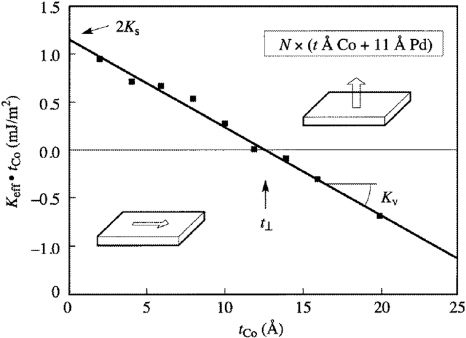
\includegraphics[scale=1.0]{surfaceandinterface}
\caption{Figure 1: Magnetic anisotropy as a function of film thickness}
\end{figure}

Due to the shape anisotropy $K^V$ is negative. This can directly be seen by the negative slope which results in an in-plane magnetization. The zero-crossing occurs at a positive value $K^S$, which leads to a critical thickness $d_c$:
\begin{equation}
d_c = -\frac{2K^2}{K^V}
\end{equation}

with
\begin{equation}
d < d_c : perpendicular magnetization
d > d_c : in-plane magnetization
\end{equation}

due to the change of sign of $K^{eff}$. Thus, the volume contribution always dominates for thick films with a magnetization being within the film plane. 

\end{document}